% !TEX TS-program = xelatex
% !TEX encoding = UTF-8 Unicode
% !Mode:: "TeX:UTF-8"

\documentclass{resume}
\usepackage{zh_CN-Adobefonts_external} % Simplified Chinese Support using external fonts (./fonts/zh_CN-Adobe/)
% \usepackage{NotoSansSC_external}
% \usepackage{NotoSerifCJKsc_external}
% \usepackage{zh_CN-Adobefonts_internal} % Simplified Chinese Support using system fonts
\usepackage{linespacing_fix} % disable extra space before next section
\usepackage{cite}
\usepackage[dvipsnames]{xcolor}
\usepackage{graphicx}
\usepackage{calc}
\usepackage[most]{tcolorbox}

\newcommand{\schooltag}[1]{%
  \tcbox[
    on line,
    boxsep=1.2pt,
    left=2pt,
    right=2pt,
    top=1pt,
    bottom=1pt,
    colback=cyan!12,
    colframe=cyan!12,
    arc=2pt,
    boxrule=0pt
  ]{\textcolor{cyan!80}{\sffamily\normalsize #1}}\hspace{4pt}%
}

% Avoid hyperref bookmark warnings when \schooltag appears in section titles.
\pdfstringdefDisableCommands{%
  \def\schooltag#1{}%
  \def\quad{ }%
}

% 收紧 section 标题的上下间距（resume.cls 默认为 *1.8/*1.8），使全文控制在一页内。
% *n 的单位为 1ex（titlesec 的 \beforetitleunit / \aftertitleunit）。
\titlespacing*{\section}{0cm}{*1.2}{*1.0}

\begin{document}
\pagenumbering{gobble} % suppress displaying page number

%左上角放置学校 logo
\noindent\makebox[0pt][l]{%
  \raisebox{-0.4\height}[0pt][0pt]{%
    
\includegraphics[width=0.28\textwidth]{hit-logo_compressed.png}%
  }%
}%

% 右上角放置照片
\noindent\hfill\raisebox{-0.6\height}[0pt][0pt]{%
  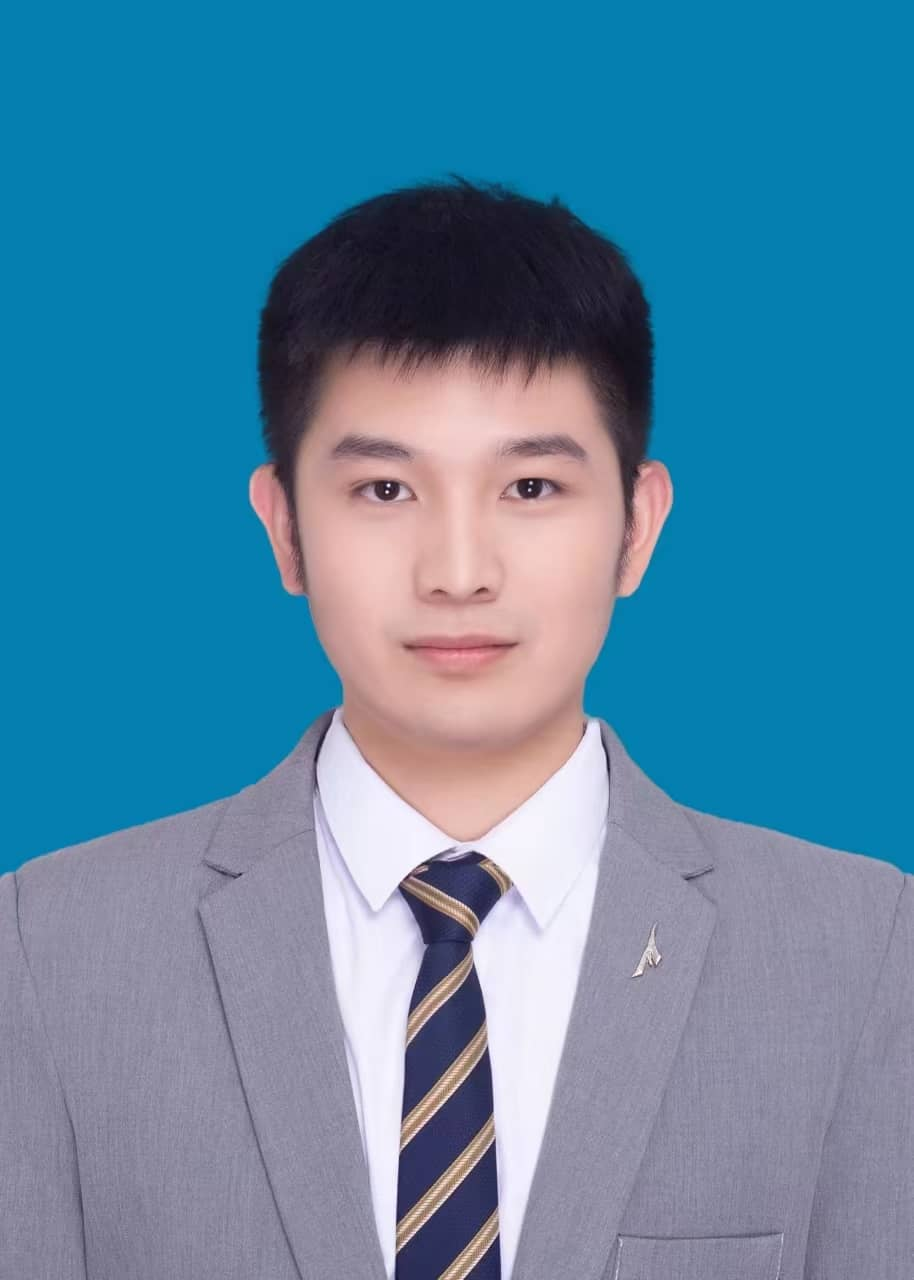
\includegraphics[width=0.95in]{freecompress-证件照（蓝）.jpg}%
}\par\vspace{-1.4em}

\name{侯金科}

\basicInfo{
  \phone{187-3619-1305}｜
  \email{2901779563@qq.com}
}\vspace{-0.3em}

\section{\texorpdfstring{\faGraduationCap\ 教育背景}{教育背景}}
\datedsubsection{\textbf{哈尔滨工业大学} \quad 电子信息 （硕士在读）\schooltag{985}\schooltag{211}\schooltag{双一流}}{2025.09 -- 至今}
\datedsubsection{\textbf{郑州大学} \quad 物联网工程 （本科） \schooltag{211}\schooltag{双一流}}{2021.09 -- 2025.06}
\textit{英语：CET-6}\quad\textit{GPA：3.63/4.00}\quad\textit{专业排名: 24/143}

\section{\texorpdfstring{\faUsers\ 项目经历}{项目经历}}
\datedsubsection{\textbf{基于Nanobot的多平台智能个人助理}\ \texorpdfstring{\href{https://github.com/Discard-001/nanobot-assistant}{\faGithub\ {\footnotesize github.com/Discard-001/nanobot-assistant}}}{}}{2026.06 -- 2026.08}
\role{Python 3.12, HKUDS/nanobot, AI Agent, Tool Calling, MCP, asyncio}{独立研究 / 核心开发}
\begin{itemize}
  \item \textbf{项目简介}：为满足个人日程管理、消息提醒及文档处理等多样化需求，基于 Nanobot 项目进行源码级二次开发，构建具备长期记忆与多任务管理能力的 QQ / 飞书智能个人助理。
  \item \textbf{三级记忆架构实现 Agent 成长性}:基于 MEMORY.md（长期注入 System Prompt）、HISTORY.jsonl（按需检索）和 Session.jsonl（会话持久化）三层结构，结合两阶段记忆固化机制，使 Agent 持续沉淀用户偏好与领域知识。
  \item \textbf{多会话管理与上下文切换}: 针对 ReAct 长对话持续堆叠导致的注意力稀释与跨任务错误关联问题，实现多会话隔离机制与TTL压缩，为不同任务维护独立上下文，支持实时切换。
  \item \textbf{工具链打通与执行过程透明化}: 打通日程管理（创建/查询/提醒）和文献检索工具链，基于飞书 CardKit 流式卡片与 QQ 流式消息 API，将思考链与工具调用按时间线交错实时外显，使 Agent 行为可解释、可追踪。
  \item \textbf{RAG 增强的PDF问答}：接入 MinerU 实现论文 PDF 结构化解析（含公式等），结合 FAISS 向量库与 BGE-M3 嵌入 / 重排序模型，构建“解析 → 检索 → 生成”端到端链路，缓解长文档截断与幻觉问题。
  \item \textbf{多模态输入输出扩展}：实现语音消息自动转写（ASR 失败自动兜底），集成图片 / 视频生成（OpenAI 兼容 API，异步任务轮询 + 限流重试，支持文生 / 图生视频），覆盖语音、图像、视频全链路。
\end{itemize}

\datedsubsection{\textbf{基于 Llama3 的轻量级大语言模型训练与对齐系统}}{2026.03 -- 2026.05}
\role{Python, PyTorch, Transformer, LoRA, DPO/GRPO}{个人项目}
\begin{itemize}
  \item \textbf{项目简介}：面向轻量级大语言模型训练场景，独立完成从模型搭建、预训练、指令微调到偏好对齐的完整实验流程，系统复现并实践小规模 LLM 训练与后训练核心方法。
  \item \textbf{从 0 搭建轻量级大语言模型}：基于 Decoder-only 架构实现轻量模型，完成 RoPE 位置编码、KV Cache、GQA 注意力、RMSNorm 等核心模块开发，为后续训练与对齐提供统一模型底座。
  \item \textbf{完成预训练与微调全流程}：基于 PyTorch 搭建预训练、SFT 和 LoRA 微调代码，支持混合精度、梯度累积；结合对话模板与 loss mask 设计，减少无效监督信号干扰，提升训练稳定性。
  \item \textbf{实现模型后训练与偏好对齐}：基于偏好数据实现 DPO、GRPO 等后训练方法，结合规则奖励与推理格式约束，提升回答一致性与推理结果的格式稳定性。
\end{itemize}


\section{\texorpdfstring{\faCogs\ 专业技能}{专业技能}}
\begin{itemize}[parsep=0.3ex, leftmargin=*]
  \item 熟悉RAG工程化落地，实践过混合检索（向量+BM25）与Rerank策略优化
  \item 熟悉Agent开发，有Function Calling工具编排与MCP协议接入经验
  \item 熟悉Prompt Engineering，掌握结构化Prompt设计与输出约束方法
  \item 熟悉向量数据库（Milvus/Weaviate），有索引调优与检索性能优化经验
  \item 了解大模型微调流程（SFT/LoRA），理解微调与RAG的选型边界
\end{itemize}

\section{\texorpdfstring{\faHeartO\ 获奖情况}{获奖情况}}
\datedline{全国大学生物联网设计竞赛（华为杯）西北赛区一等奖、全国总决赛三等奖}{2023}
\datedline{蓝桥杯全国软件和信息技术专业人才大赛河南赛区 C/C++ 程序设计大学 A 组二等奖}{2023}
% \datedline{网络技术挑战赛华中赛区三等奖}{2023、2024}
% \datedline{郑州大学优秀学生奖学金二等奖（3 次）}{2022、2023、2024}
\datedline{计算机软件著作权 2 项}{2024}
% \datedline{郑州大学 2022--2023 学年三好学生}{2023}

\end{document}
